% Determines the type of document and font size
\documentclass[12pt,a4paper]{article}
% Font control
\usepackage{mathptmx} % Times Roman Font
\usepackage{helvet} % Arial/Helvetica font
\renewcommand{\familydefault}{\sfdefault} % Makes serif text all Helvetica
% Set up the page margins
\usepackage[left=2.5cm, right=2.5cm, top=2.5cm]{geometry}
% set the line space to 1.5
\usepackage{setspace}
\onehalfspacing
% Allow graphics
\usepackage{graphicx}
% put graphs in place
\usepackage[section]{placeins}
% caption font
\usepackage[font=small,labelfont=bf]{caption}
% float package: picture position
\usepackage{float}
% symbols
\usepackage{textcomp, gensymb}
% hyperref
\usepackage{hyperref}
% Add your report title here
\title{OCNG/ATMO 651 Final Project: Linear Inverse Model of Tropical Sea Surface Temperatures}
% Add your name here
\author{Jinjun Liu}
\date{\today}

% The start of the document
\begin{document}
% This adds the title page
\maketitle
\thispagestyle{empty}
% This adds the abstract
\begin{abstract}

In this project, we employ the linear inverse model (LIM) to predict sea surface tempratures anomalies (SSTAs) in the global tropics. The LIM is based on the empirical orthogonal function (EOF) decomposition of the SSTAs. We use the monthly NCEP/NCAR reanalysis SST as the dataset to build the LIM and make predictions. The LIM is more skillful well when the leading time is not large. The tropical averaging correlation coefficient can reach to 0.54 when the leading time is one month. The LIM performs well in the Ni\~no 3 region and Indian Ocean, but not very well in the tropical Atlantic and northwest Pacific. The LIM forecast based on the latest SST observations suggest that the La Ni\~na event will likely continue in the next few months.

\end{abstract}

\tableofcontents

% Move to a new page and set the page numbering from here
\clearpage % moves to the next page
\pagenumbering{arabic}

\section{Introduction} % The start of a new section

Sea surface temperatures (SSTs) are important for ocean and atmosphere because they play a significant role in shaping the Earth's climate and weather patterns. Many climate variability modes are directly related to the SSTs. For example, the El Ni\~no-Southern Oscillation (ENSO) is a coupled ocean-atmosphere phenomenon that is characterized by the fluctuation of warming and cooling of the central and eastern equatorial Pacific Ocean \cite{McPhaden2006}. The Atlantic Multidecadal Oscillation (AMO) is a long-term observed climate variability mode that is characterized by altering the warming and cooling phases of the North Atlantic SSTs in multi-decadal time scale \cite{Knight2006}. These large-scale climate variability not only affect the global climate but also have a significant impact on the regional climate and weather patterns (e.g., IPCC AR5 \cite{christensen2013climate}). Therefore, it is important to predict the SST future changes in order to make climate predictions.

Penland and Magorian \cite{Penland1993} and Penland and Matrosova \cite{Penland1998} proposed a linear inverse model (LIM) to predict the SSTs in the region of the equatorial Pacific Ocean and Tropical Atlantic. This method is based on the empirical orthogonal function (EOF) decomposition of the SSTs. They found that the LIM can predict the SSTs in the region of the equatorial Pacific Ocean with a root mean square error (RMSE) of half a degree Celcius when the leading time of 9 months is used. In the Caribbean Sea and north tropical Atlantic, Penland and Matrosova \cite{Penland1998} found that the LIM can predict the SSTs better when using the global tropical SSTs as predictors compared only using tropical Atlantic SSTs as predictors. They also found that the SST anomaly in the Ni\~no 3 region is a strong 6-month predictor of SST anomaly in the north tropical Atlantic. Penland \cite{Penland1996} stated that the "optimal initial structure" predicted by LIM is approximately seven months before most of the major warm and cold (El Ni\~no/La Ni\~na) events in the data record.

Richter el al. \cite{Richter2020} examine the impact of impacs of general circulation models (GCMs) errors on prediction skill as estimated by the LIM. It is found that the observation-derived LIM is more skillful than a simple persistence forecasts in most regions. Its skill also compares well with some GCM forecasts except in the equatorial Pacific, where the GCMs are superior. This indicates that the LIM performs well even compared with the complicated GCMs.

In this project, we employ the LIM to predict the SST anomalies (SSTAs) in the global tropics. The detailed method of the LIM is described in Section \ref{dataset-method}. The results of the LIM are shown in Section \ref{results}. The discussion and conclusion are presented in Section \ref{conclusion}.

\section{Dataset and Method}\label{dataset-method}

We use the NCEP/NCAR (National Centers for Environmental Prediction/National Center for Atmospheric Research) reanalysis SST as the dataset to build the LIM and make predictions. This dataset used in this project contains monthly-mean SSTs from January 1948 to September 2017. We divide the dataset into two parts: the training dataset and the test dataset. The training dataset contains the SSTs from January 1948 to December 1999, and the test dataset contains the SSTs from January 2000 to September 2017. We use the training dataset to build the LIM and use the test dataset to evaluate the performance of the LIM.

The latest SST observations (November 2022) is obtained from the monthly COBE SST (Daily Sea Surface Analysis for Climate Monitoring and Predictions) dataset \cite{Ishii2005}. Horizontal resolution of COBE SST is 1.0$^{\circ}$. To use the LIM built from the NCEP/NCAR reanalysis SST, we interpolate the COBE SST to the same grid as the NCEP/NCAR reanalysis SST. The interpolation is done by using the bilinear interpolation method.

The LIM assumes that the time evolution of the SSTs can be described as a linear differential equation:

\begin{equation}
\label{eq:lim}
\frac{d\mathbf{T}}{dt} = \mathbf{A} \mathbf{T} + \xi
\end{equation}

where $\mathbf{T}$ is the SST vector, $\mathbf{A}$ is the linear operator, and $\xi$ is the noise. The LIM assumes that the noise $\xi$ is small and can be neglected. Then the evolution of $\mathbf{T}$ from time $t$ to time $t+\Delta t$ can be approximated as:

\begin{equation}
\label{eq:lim-2}
\mathbf{T}(t+\Delta t) = e^{\mathbf{A}\Delta t} \mathbf{T}(t) + \epsilon
\end{equation}

where $e^{\mathbf{A}\Delta t}$ is called the propagator matrix, and $\epsilon$ is the noise. By left-multiplying the tranpose of SST vector $T' (t)$ on both sides of Eq. (\ref{eq:lim-2}), we have:

\begin{equation}
\label{eq:lim-3}
<T(t+\Delta t) T'(t)> = e^{\mathbf{A}\Delta t} <T(t) T'(t)> + <\epsilon T'(t)>
\end{equation}

where $<\cdot>$ denotes the time average. $T(t)T'(t) = \mathbf{C}$ is the covirance matrix of the SSTs. $T(t+\Delta t)T'(t) = C_{\Delta t}$ is the lag-covirance at $\Delta t$. If we neglect the noise term, we have:

\begin{equation}
\label{eq:lim-4}
C_{\Delta t} = e^{\mathbf{A}\Delta t} \mathbf{C}
\end{equation}

Then the propagator can be determined as:

\begin{equation}
\label{eq:lim-5}
\mathbf{G}=e^{\mathbf{A}\Delta t} = C_{\Delta t} \mathbf{C}^{-1}
\end{equation}

Once we have constructed the propagator matrix $G$ from the observational data, we can use it to predict the SSTs in the future. The prediction of the SSTs at time $t+\Delta t$ is given by:

\begin{equation}
\label{eq:lim-6}
\mathbf{T}(t+\Delta t) = \mathbf{G} ^{\frac{t_n - t_0}{\Delta t}} \mathbf{T}(t_0)
\end{equation}

where $t_0$ is the initial time, $t_n$ is the prediction time, and $\Delta t$ is the lag time. According to Penland and Magorian \cite{Penland1993}, we take the lag time as 7 months. However, the physical space of SST could be too large, making it difficult to estimate the propagator matrix. Therefore, we construct the LIM in EOF space. The EOF decomposition of the SSTs can be written as:

\begin{equation}
\label{eq:eof}
\mathbf{T}(t) = \sum_{i=1}^M P_i(t) \mathbf{E}_i,
\end{equation}
    
where $\mathbf{T}(t)$ is the SST vector, $P_i(t)$ is the principal components (PCs) of the $i$th EOF mode, and $\mathbf{E}_i$ is the $i$th EOF mode. $M$ is the total number of EOF modes. In EOF space, the LIM can be written as:

\begin{equation}
\label{eq:eof-lim}
\mathbf{P}(t+\Delta t) = \mathbf{G} ^{\frac{t_n - t_0}{\Delta t}} \mathbf{P}(t_0)
\end{equation}

where $\mathbf{P}(t)$ is the PCs of the EOF modes. After predicting the PCs of the EOF modes, we can reconstruct the SST vector by Eq. (\ref{eq:eof}).

The operational steps are listed as follows:

1. Smooth SST anomalies (SSTAs) using a 3-month running mean and then perform an EOF analysis on the smoothed SSTAs;

2. Reconstruct and truncate SSTAs using leading EOFs and the corresponding principal component time series as Eq. \ref{eq:eof}. Typically, $M$ is less than 10 and can be determined by the explained variance, say 90\%, by the first $M$ EOFs;

3. Compute covariance $\mathbf{\check{C}}$ and lag-covariance $\mathbf{\check{C}}_{\Delta t}$ matrix in EOF space. $\mathbf{\check{C}} = <\mathbf{P}(t) \mathbf{P}'(t)>$ and $\mathbf{\check{C}}_{\Delta t} = <\mathbf{P}(t+\Delta t) \mathbf{P}'(t)>$;

4. Compute the propagator in EOF space, $\mathbf{G}=\mathbf{\check{C}}_{\Delta t} \mathbf{\check{C}}^{-1}$, where the lag $\Delta t$ can be taken to be 7 months and $\mathbf{G}$ has $M\times M$ dimension;

5. Take an initial SSTA state vector $\mathbf{T}$ at any $t_0$, regress $\mathbf{T}(t_0)$ onto $\mathbf{E}_i$ to determine $\mathbf{P}_i(t_0)$ and then form $\mathbf{P}(t_0)$;

6. Make SST forecast in EOF space from $t_0$ to $t_n$: $\mathbf{P}(t_n) = \mathbf{G}^{\frac{t_n-t_0}{\Delta t}}\mathbf{P}(t_0)$;

7. Transform the forecast in EOF space, $\mathbf{P}(t_n)$, back to the physical space: $\mathbf{T}(t_n)=\sum _{i=1}^M \mathbf{P}(t_n) \mathbf{E}_i$.

The Python script that processes the data and generates the figures is submitted as a supplementary file.

\section{Results}\label{results}

\subsection{EOF decomposition of SSTs}\label{eof-decomposition}

\begin{figure}[htbp]
\centering
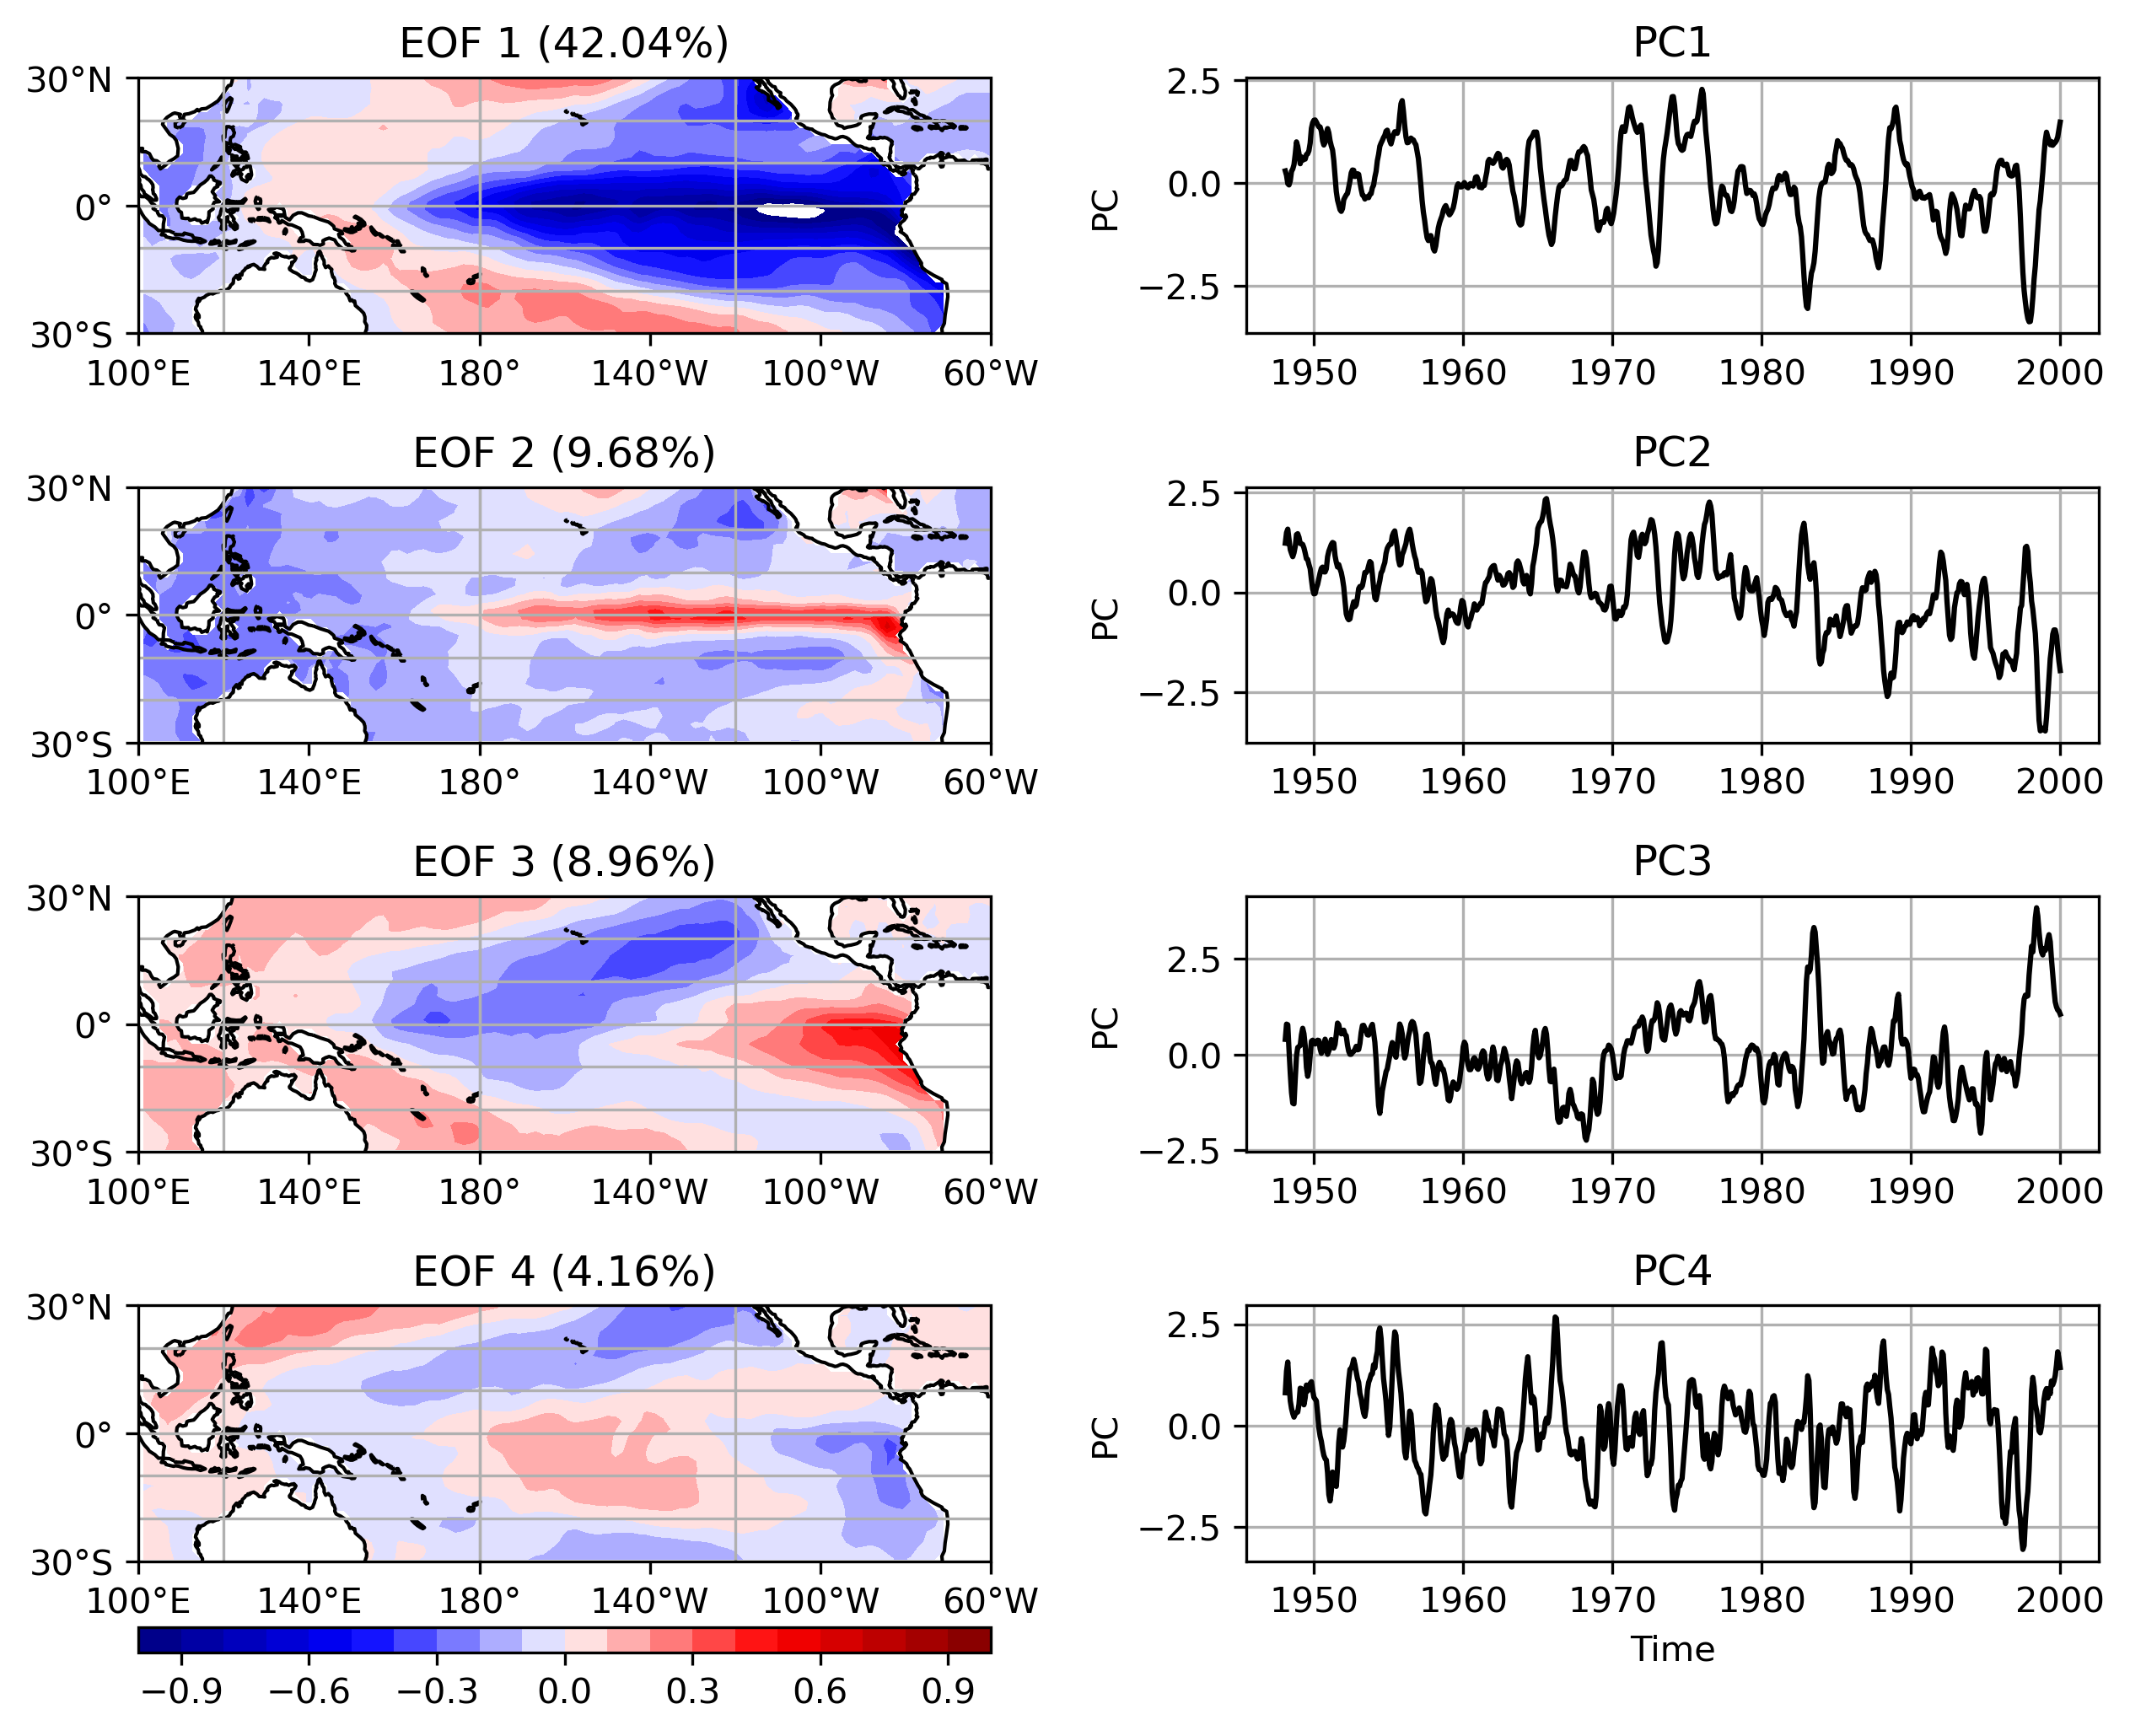
\includegraphics[width=\textwidth]{figures/EOFs_PCs.png}
\caption{EOF decomposition of SSTs.}
\label{fig:EOFs_PCs}
\end{figure}

\begin{figure}
\centering
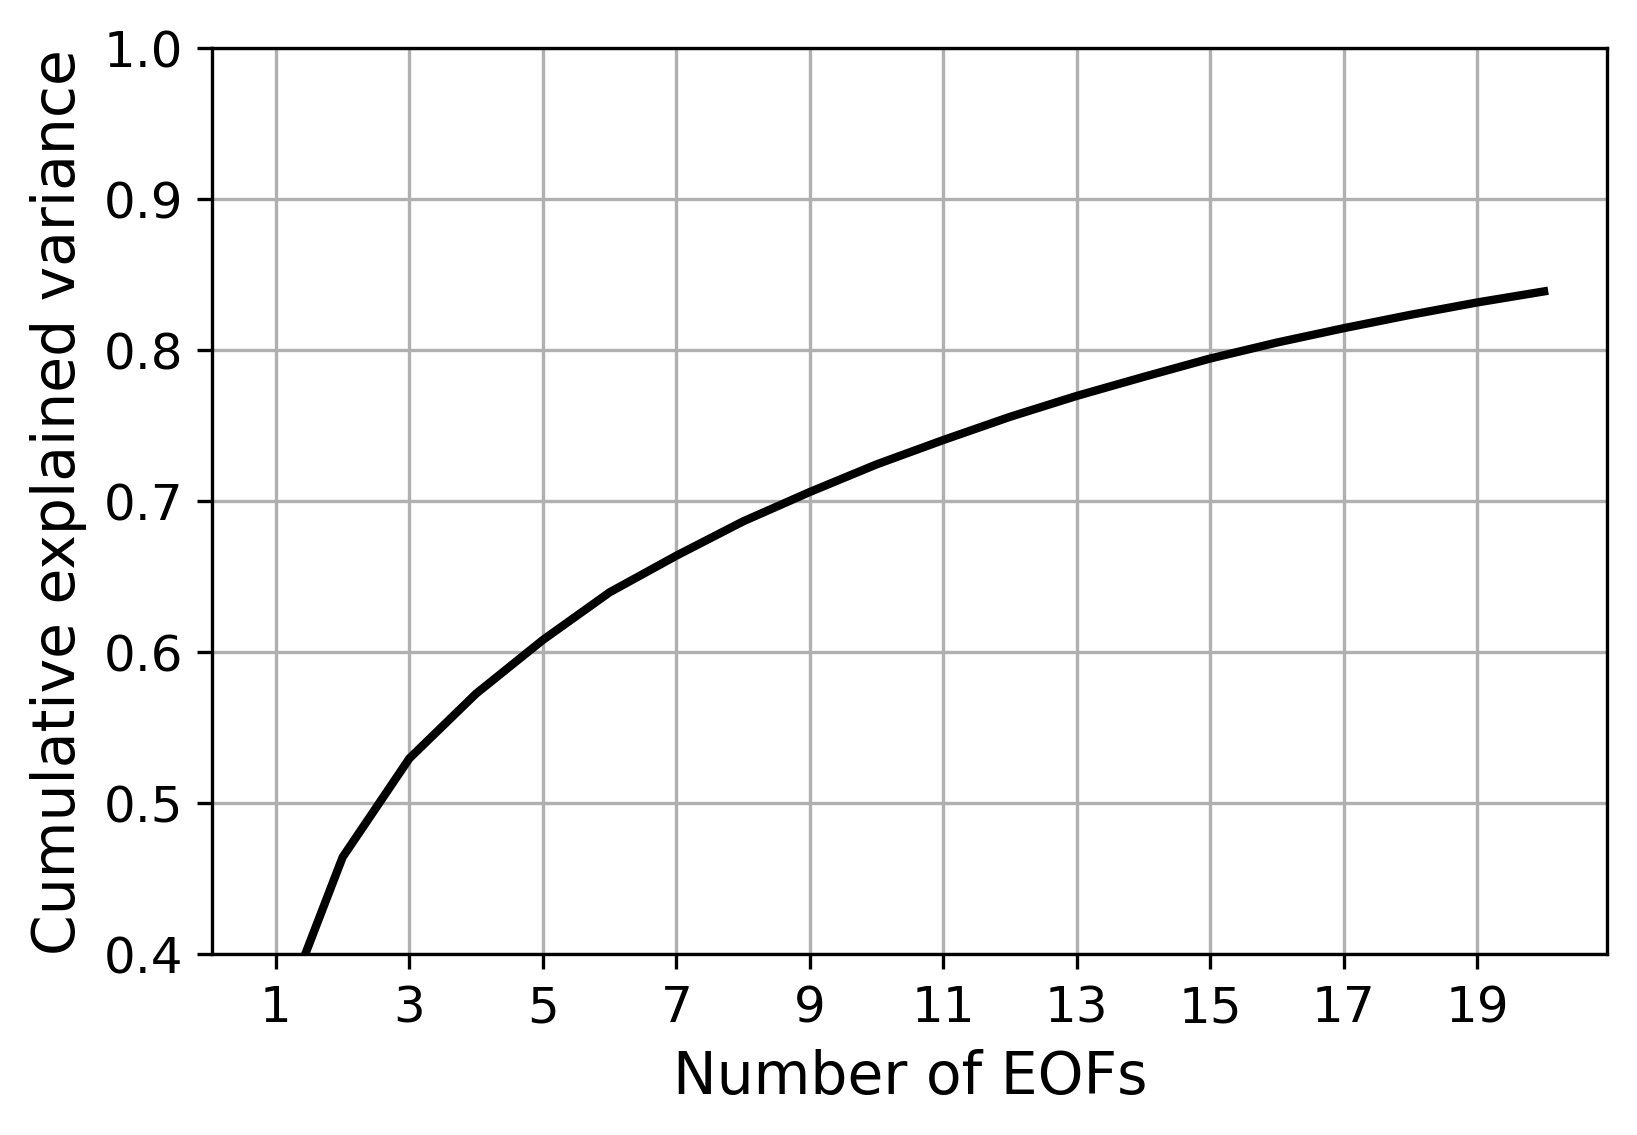
\includegraphics[width=\textwidth]{figures/cumulative_explained_variance.png}
\caption{Cumulative explained variance of the first 20 EOFs.}
\label{fig:cumulative_explained_variance}
\end{figure}

\begin{figure}
\centering
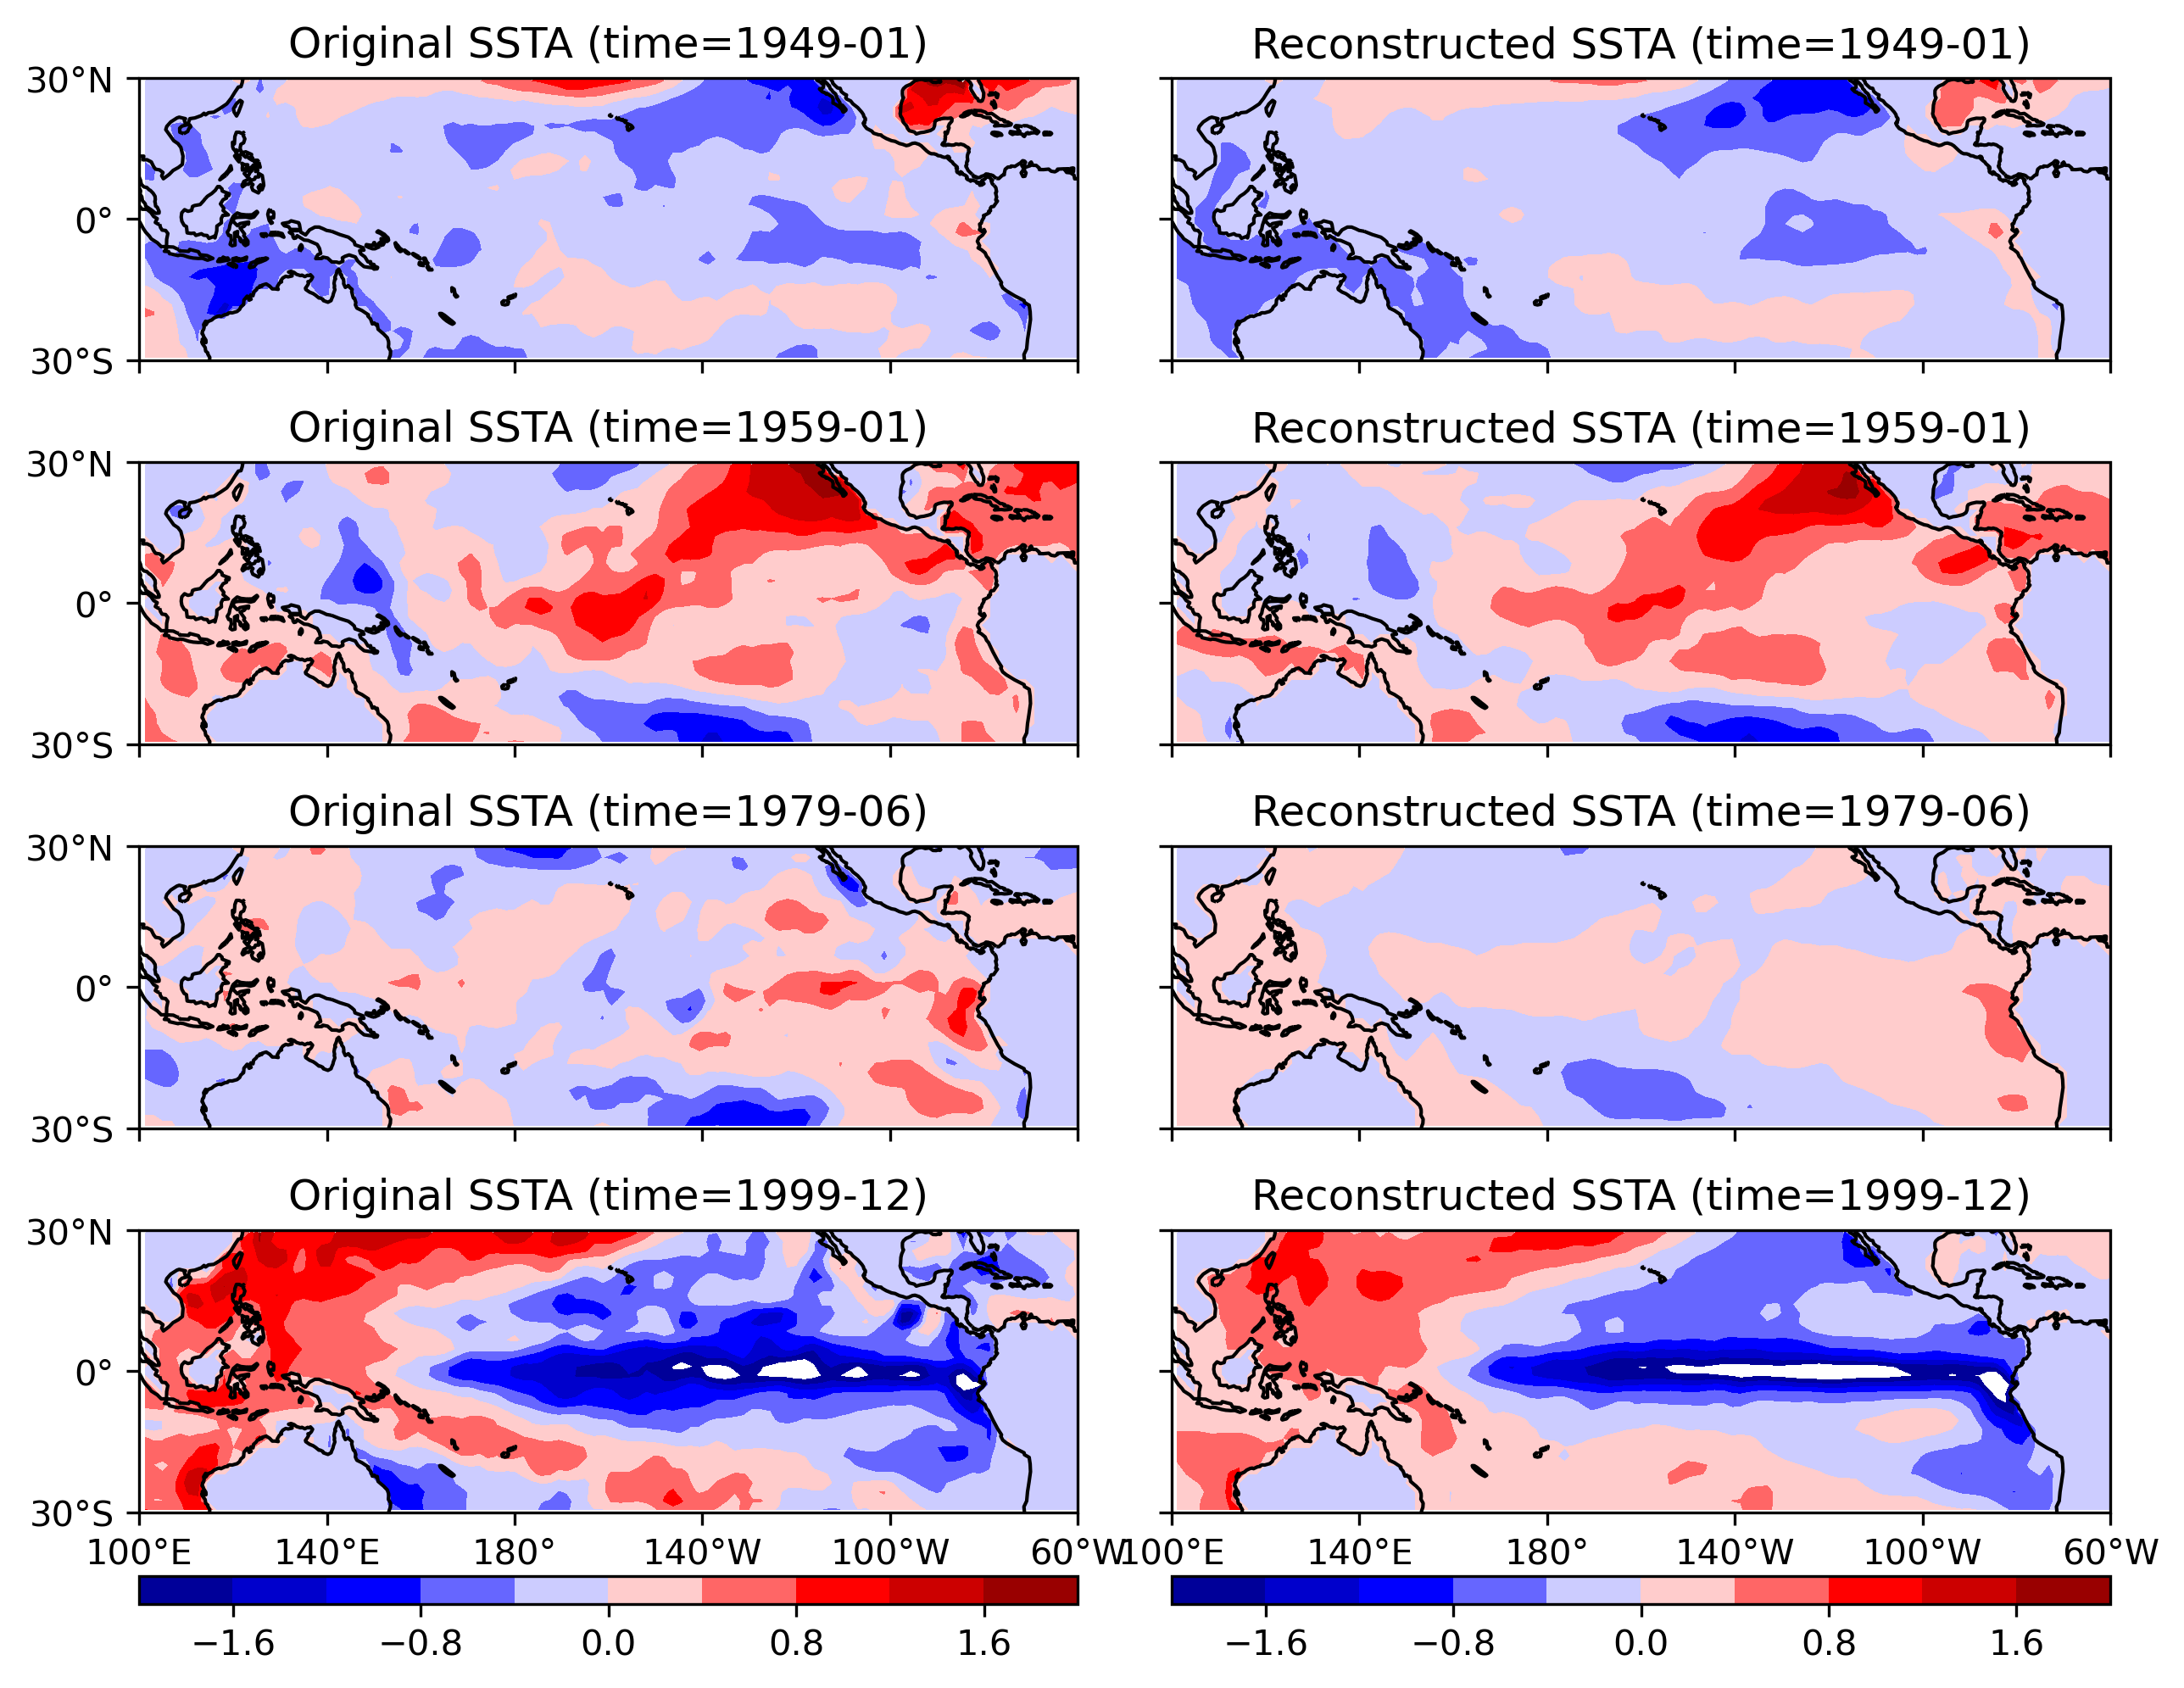
\includegraphics[width=\textwidth]{figures/reconstruct_ssta.png}
\caption{Reconstructed SSTAs using the first 15 EOFs.}
\label{fig:reconstruct_ssta}
\end{figure}

The leading four EOFs and PCs are plotted in Fig. \ref{fig:EOFs_PCs}. The first EOF mode explains 34.95\% of the variance of the SSTAs, and the second EOF mode explains 11.47\% of the variance of the SSTAs. The first 10 EOFs can explain 72.43\% of the variance of the SSTAs, the first 15 EOFs can explain 79.45\% of the variance of the SSTAs, and the first 20 EOFs can explain 83.89\% of the variance of the SSTAs (Fig. \ref{fig:cumulative_explained_variance}). When the EOF number reaches 15, the cumulative explained variance is 79.45\%, which is close to the 80\% threshold. Therefore, we choose the first 15 EOFs to reconstruct the SSTAs.

To test if the first 15 EOFs can reconstruct the SSTAs, we reconstruct the SSTAs using the first 15 EOFs and corresponding PCs and plot the reconstructed SSTAs in Fig. \ref{fig:reconstruct_ssta}. We selected four times spanning from 1949-01 to 1999-12 and varies in months. The reconstructed SSTAs are very similar to the original SSTAs, which indicates that the first 15 EOFs can reconstruct the SSTAs.

\subsection{Linear inverse model in EOF space}\label{lim-eof-space}

\begin{figure}
\centering
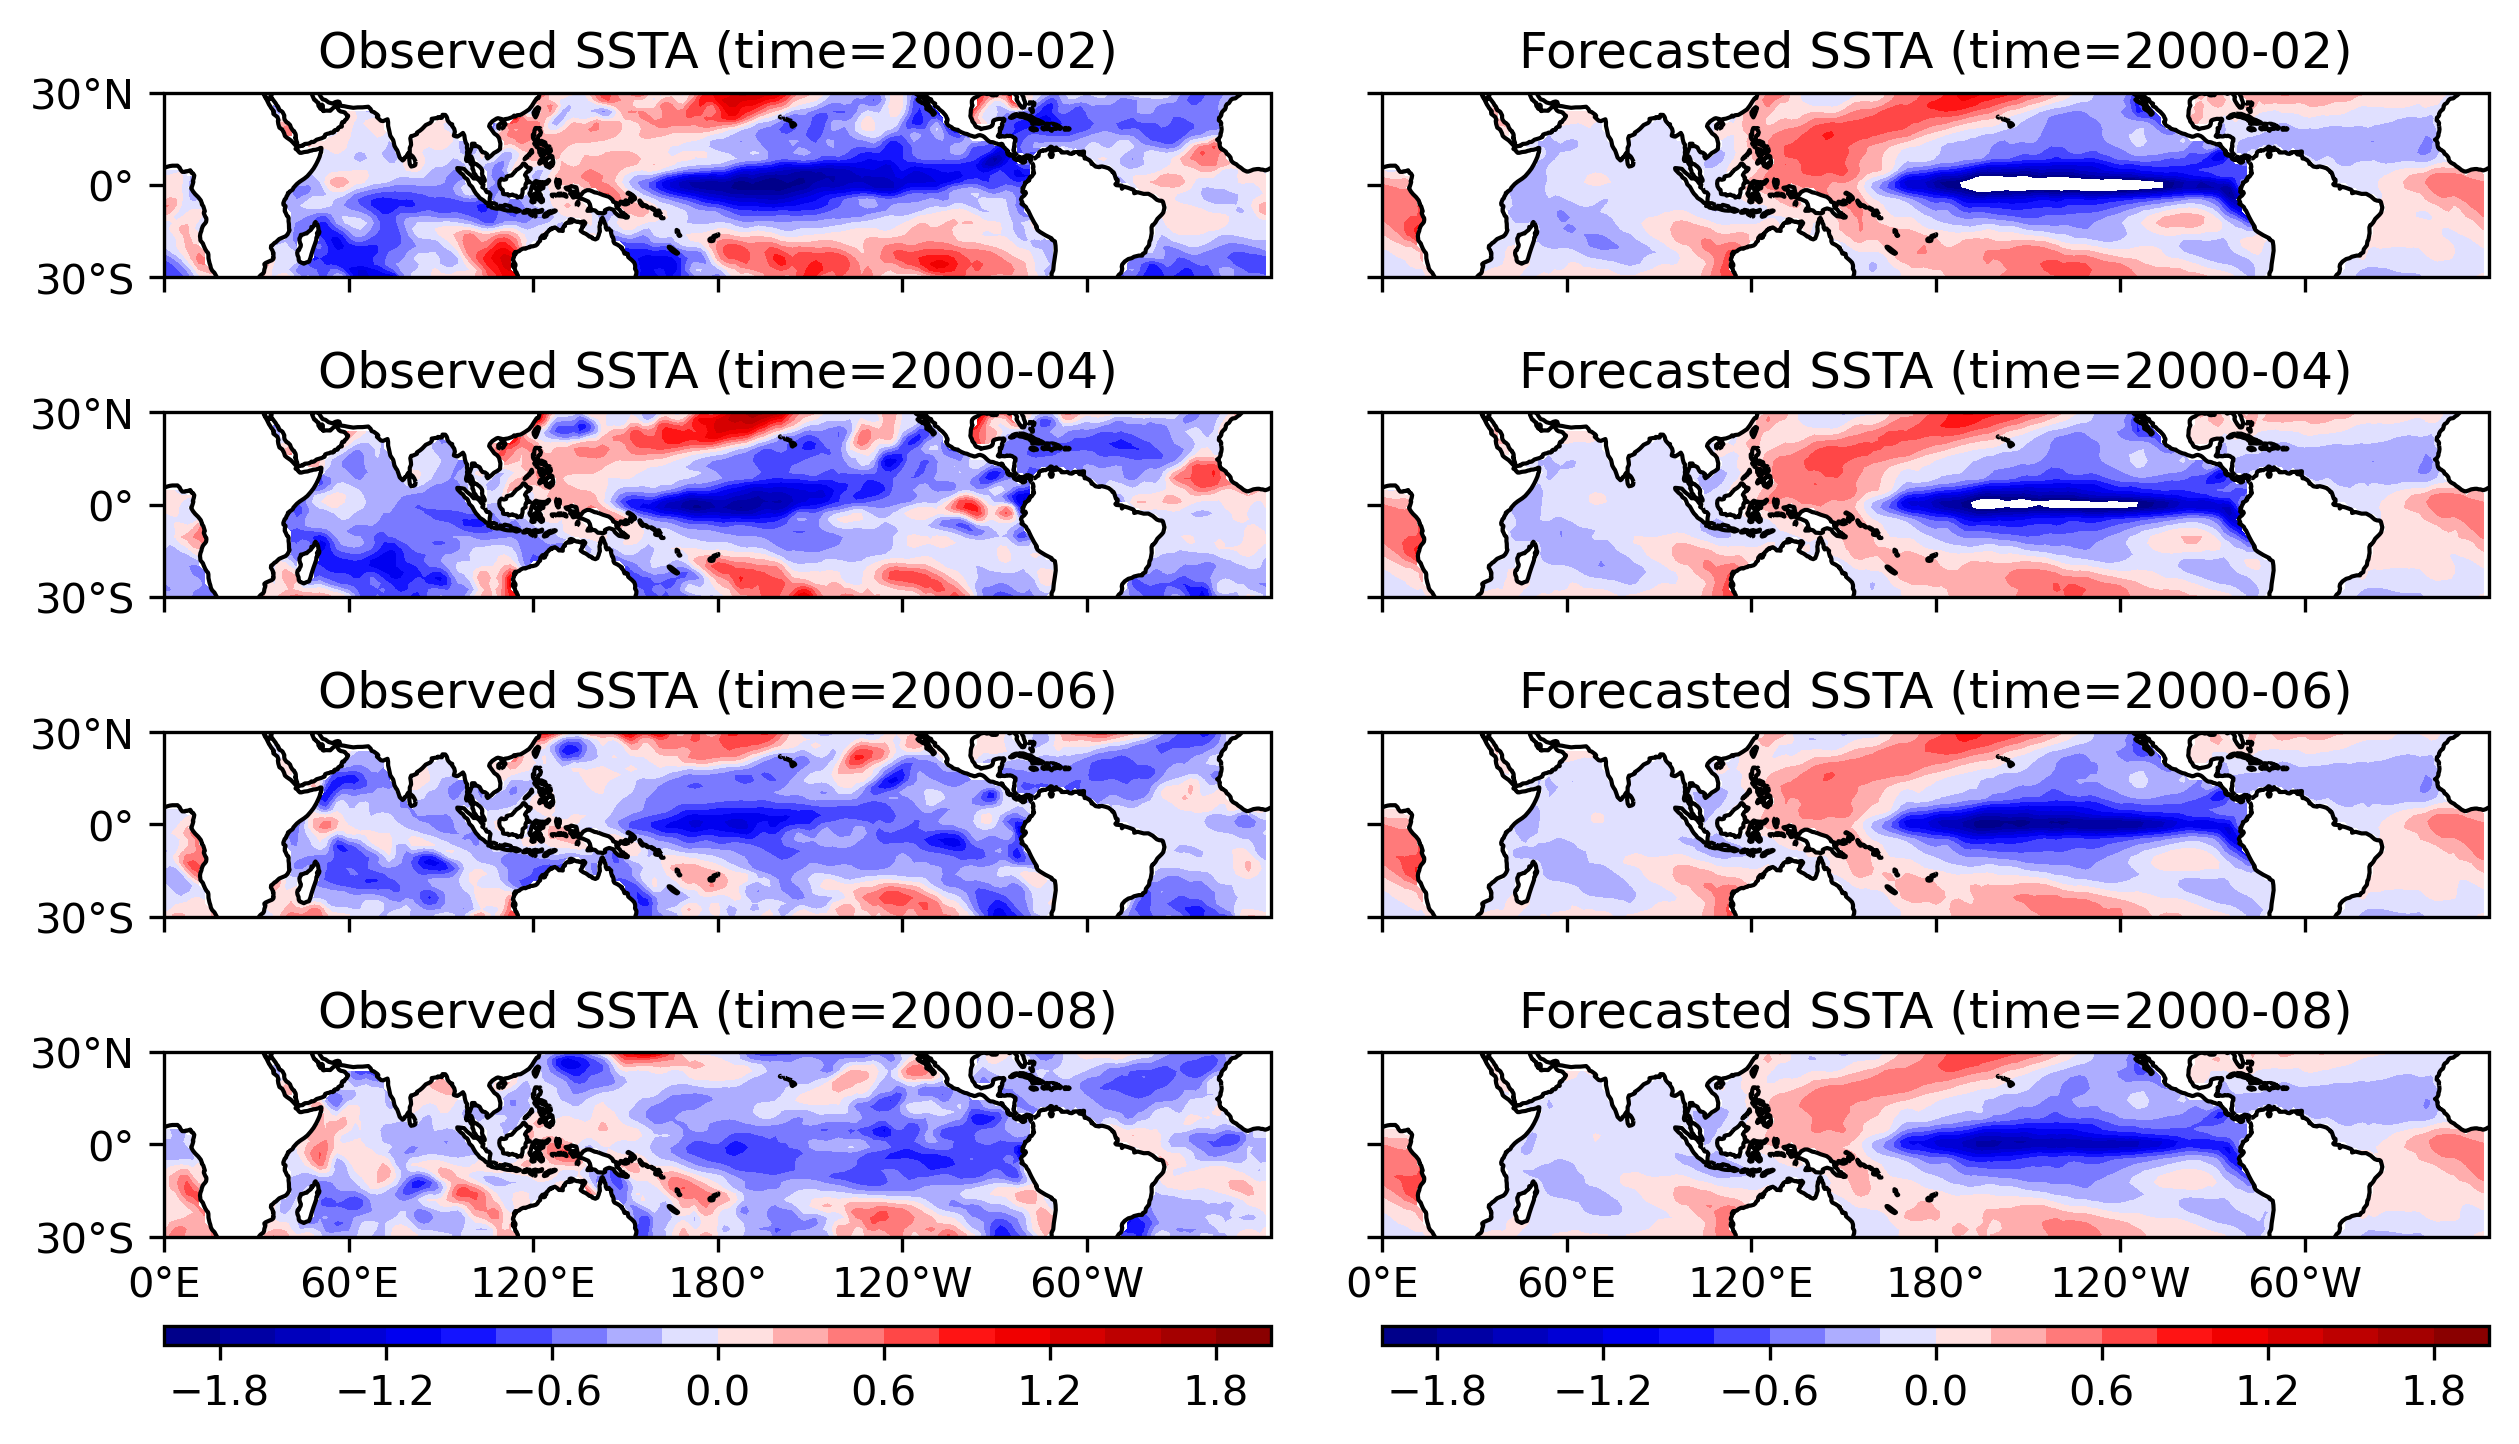
\includegraphics[width=\textwidth]{figures/forecasted_ssta_2000.png}
\caption{Forecasted SSTAs in 2000.}
\label{fig:forecasted_ssta_2000}
\end{figure}

\begin{figure}
\centering
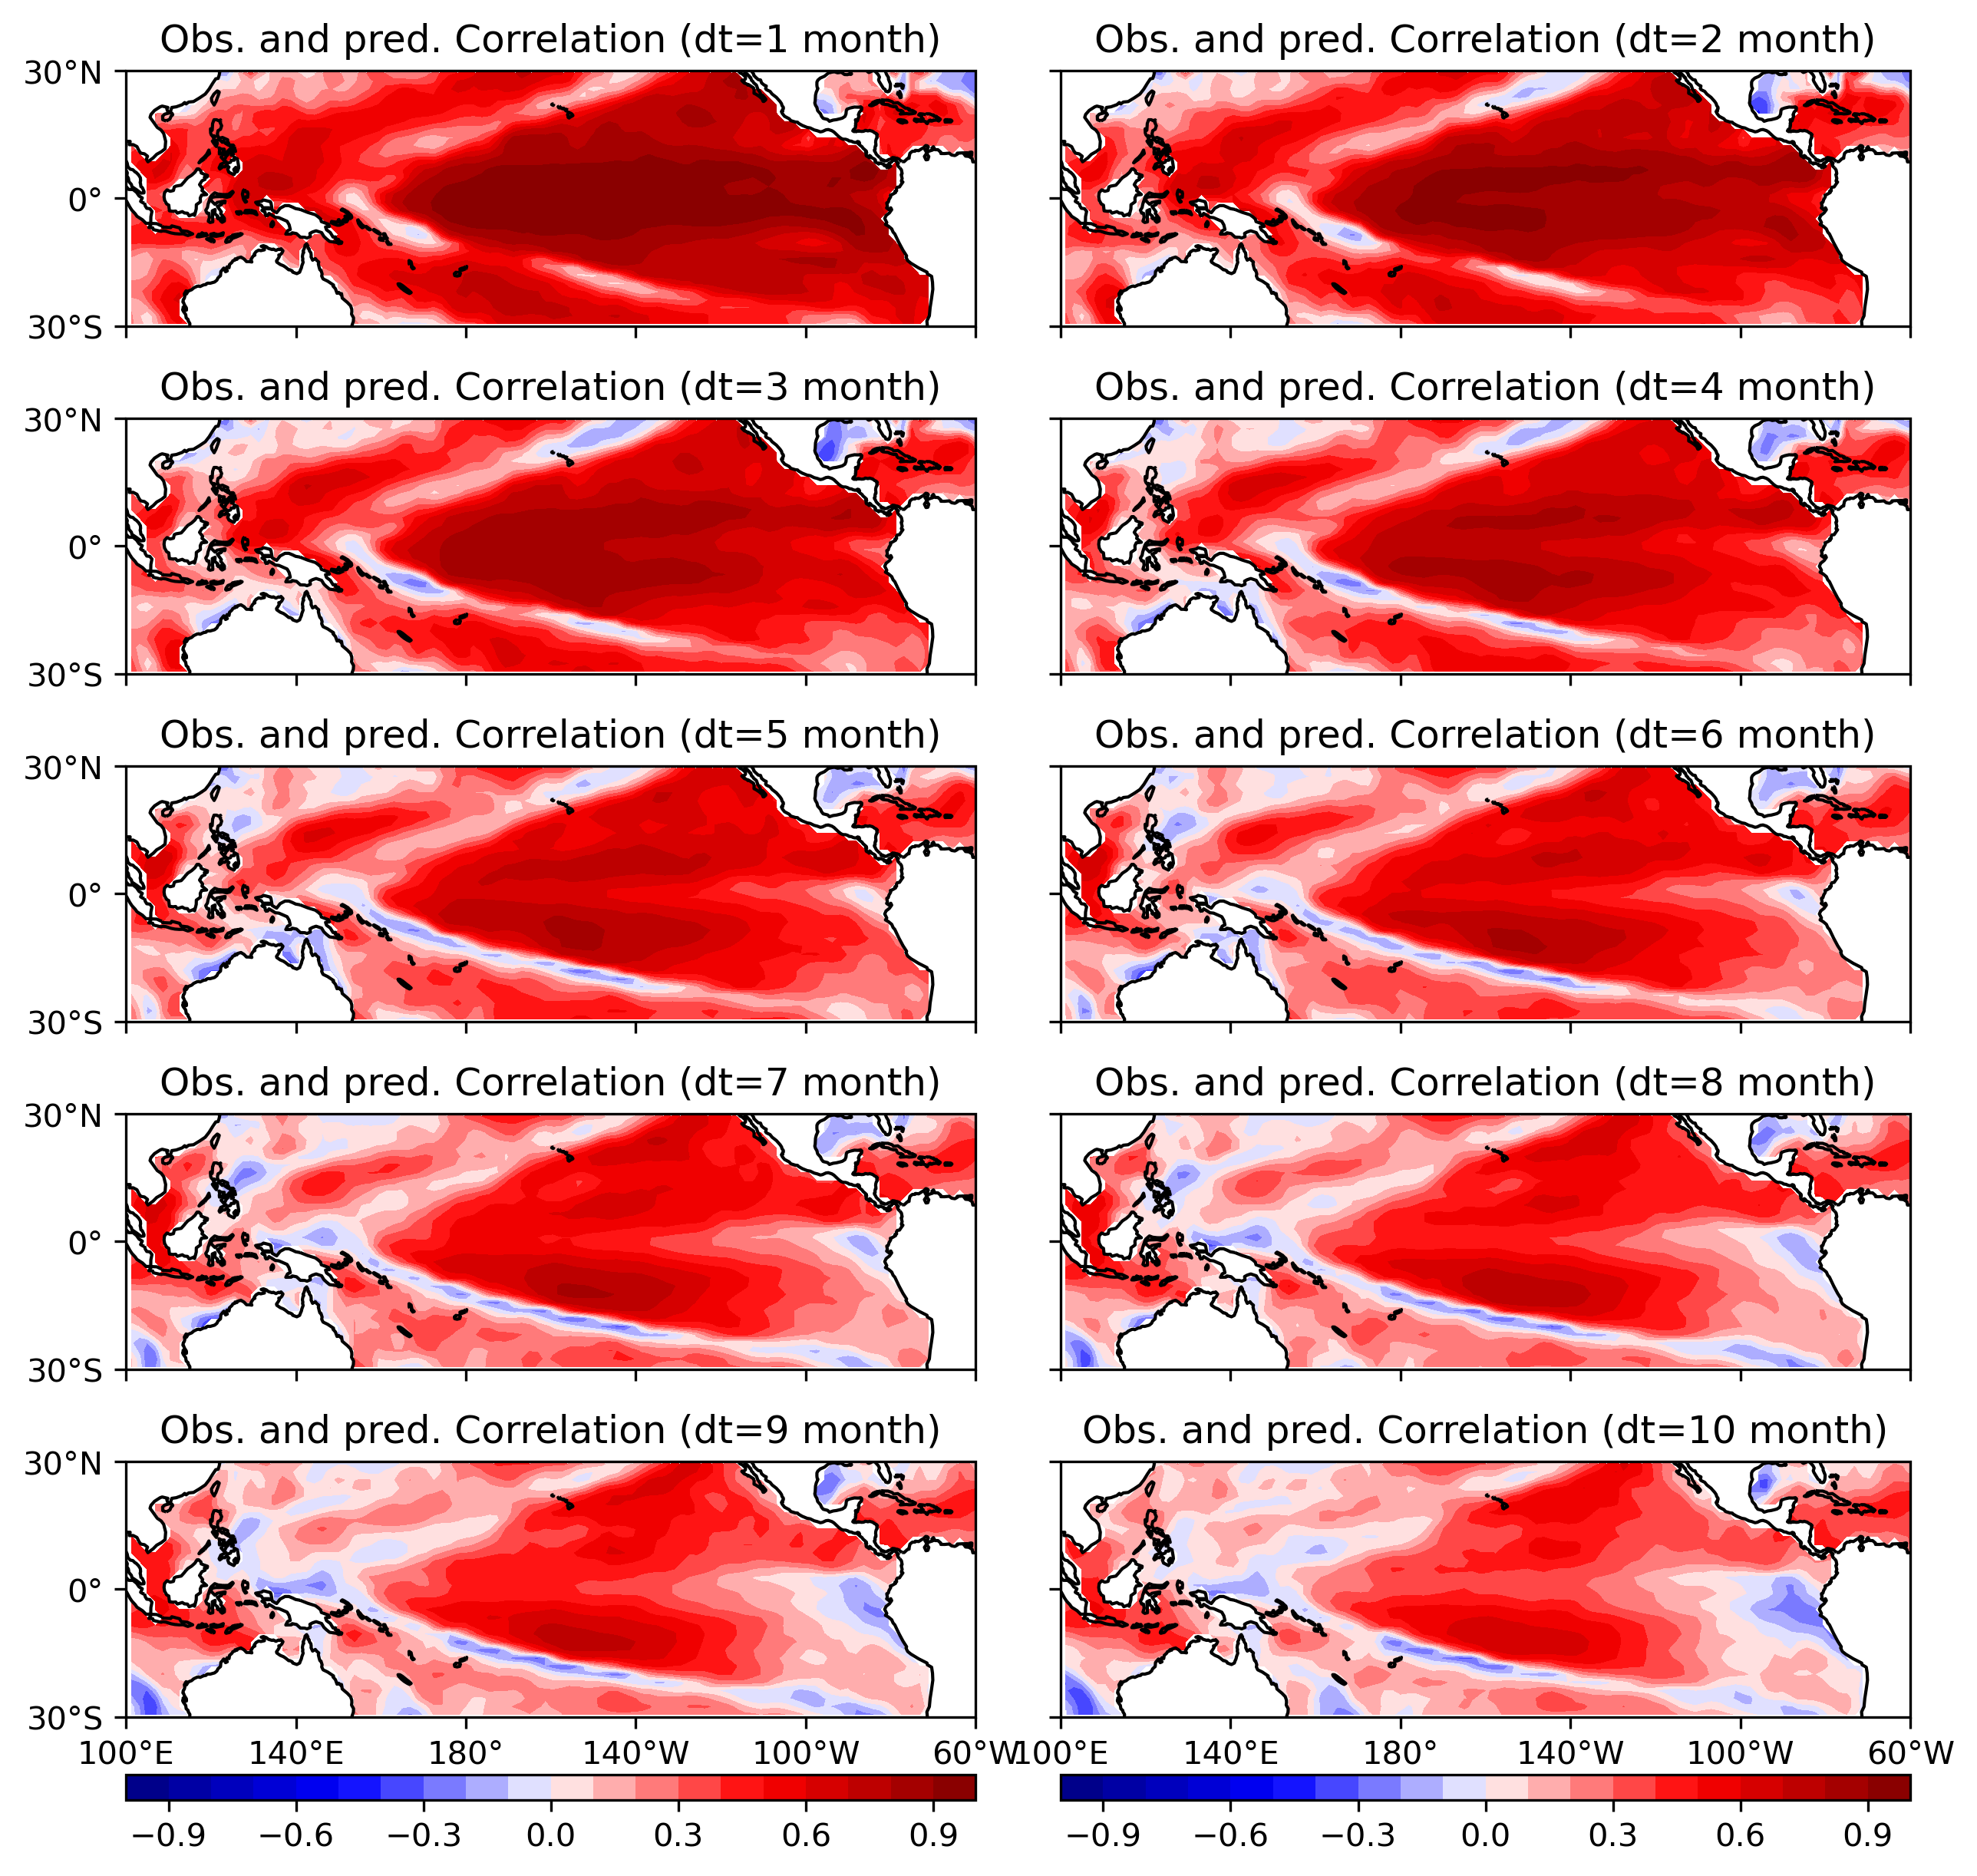
\includegraphics[width=\textwidth]{figures/corre_at_diff_leading_time.png}
\caption{Correlation between the forecasted SSTAs and the observed SSTAs at different leading times.}
\label{fig:corre_at_diff_leading_time}
\end{figure}

\begin{figure}
\centering
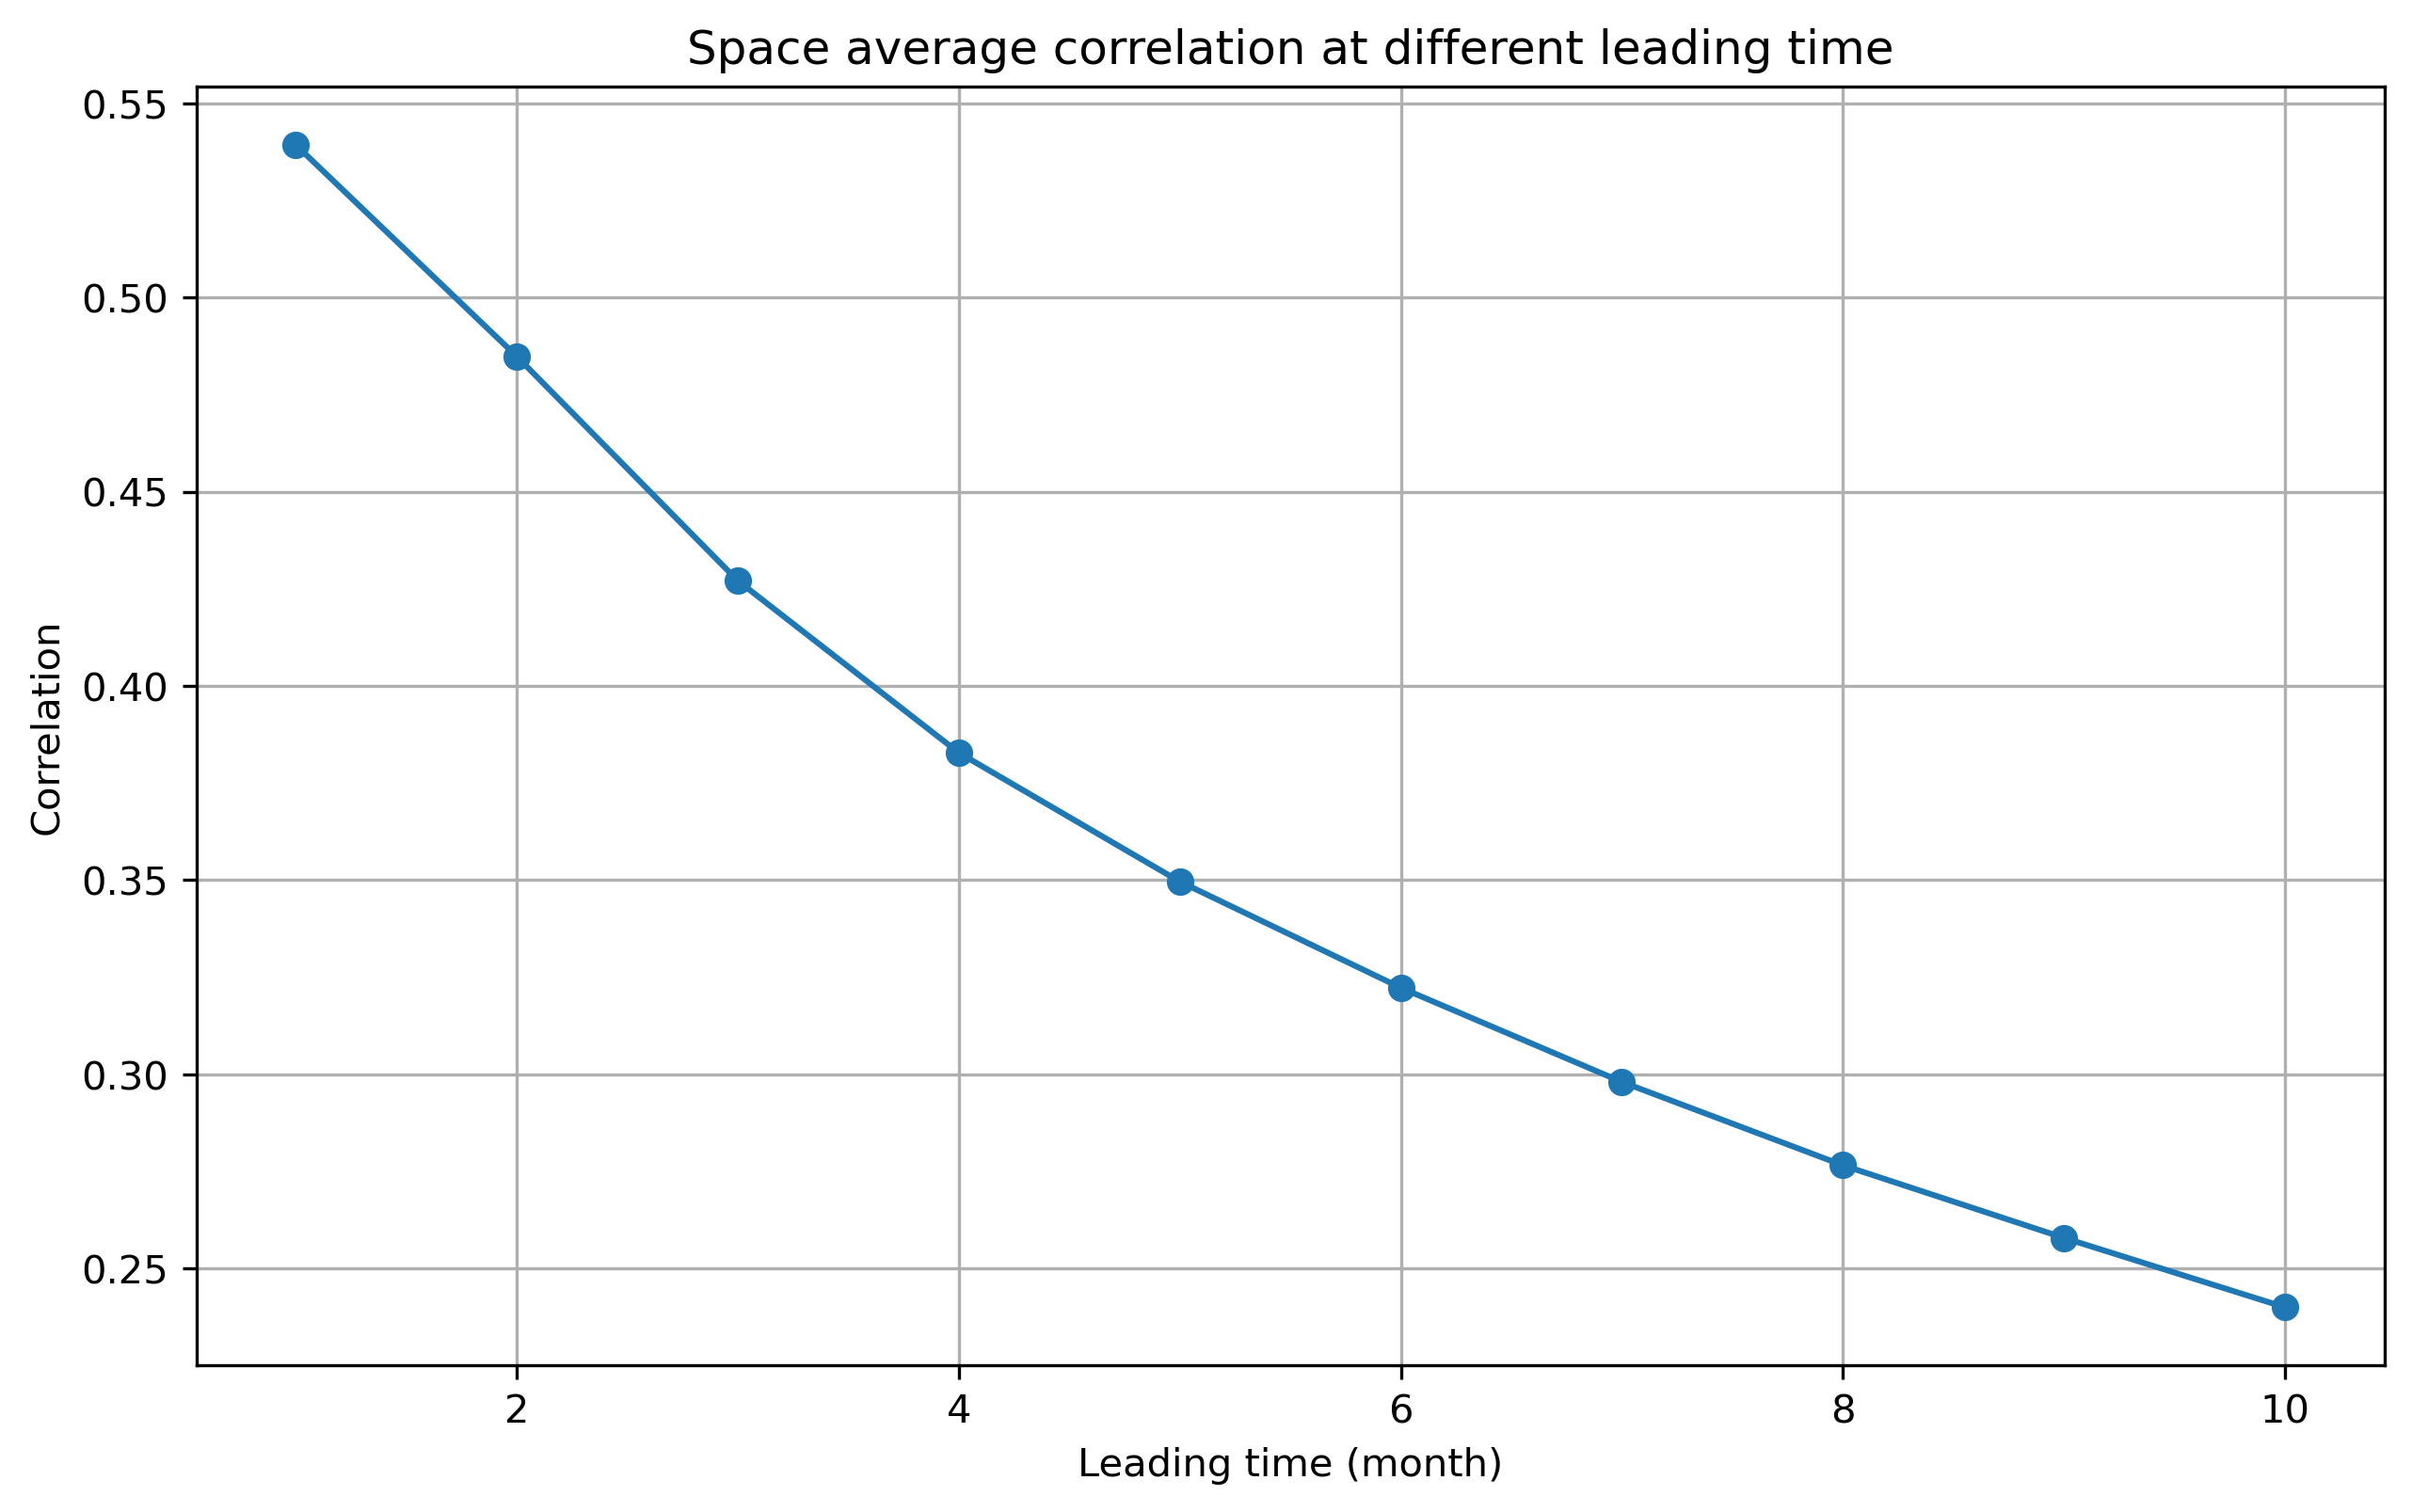
\includegraphics[width=\textwidth]{figures/corre_at_diff_leading_time_mean.png}
\caption{Space mean correlation between the forecasted SSTAs and the observed SSTAs at different leading times.}
\label{fig:corre_at_diff_leading_time_mean}
\end{figure}

We use the training data (1949-01 to 1999-12) to build the LIM. To test the performance of the model, we firstly picked 2000-01 as the initial time to apply LIM to predict the following 10 months SSTAs. The forecasted SSTAs are plotted in Fig. \ref{fig:forecasted_ssta_2000} (only 4 forecasted SSTAs are plotted). Compared to the observed SSTAs, the forecasted SSTAs are very similar to the observed SSTAs in the first a few (< 3) months. However, the forecasted SSTAs are not as good as the observed SSTAs in the later months. Therefore, the LIM is accurate when forecasting the near future SSTAs, but not accurate when forecasting the far future SSTAs.

To systematically evaluate how the leading time would influence the performance of the LIM, we calculated the correlation between the forecasted SSTAs and the observed SSTAs at different leading times. The correlation maps are plotted in Fig. \ref{fig:corre_at_diff_leading_time}. In general, the correlation is pretty high in the Ni\~no 3 region even the leading time is large. The LIM also performs well in the Indian Ocean. However, the LIM performs poorly in the north Atlantic (especially in the Mexico Gulf) and tropical Atlantic. In the Northwest Pacific, the LIM also perform poorly.

When the leading time increases, the correlation decreases. Fig. \ref{fig:corre_at_diff_leading_time_mean} shows the space mean correlation between the forecasted SSTAs and the observed SSTAs at different leading times. The space mean correlation monotonically decreases with the leading time. The correlation is the highest when the leading time is 1 month (about 0.54), and the correlation is the lowest when the leading time is 10 months (about 0.23).

\subsection{Prediction based on latest SSTs}\label{prediction-latest-ssts}

\begin{figure}
\centering
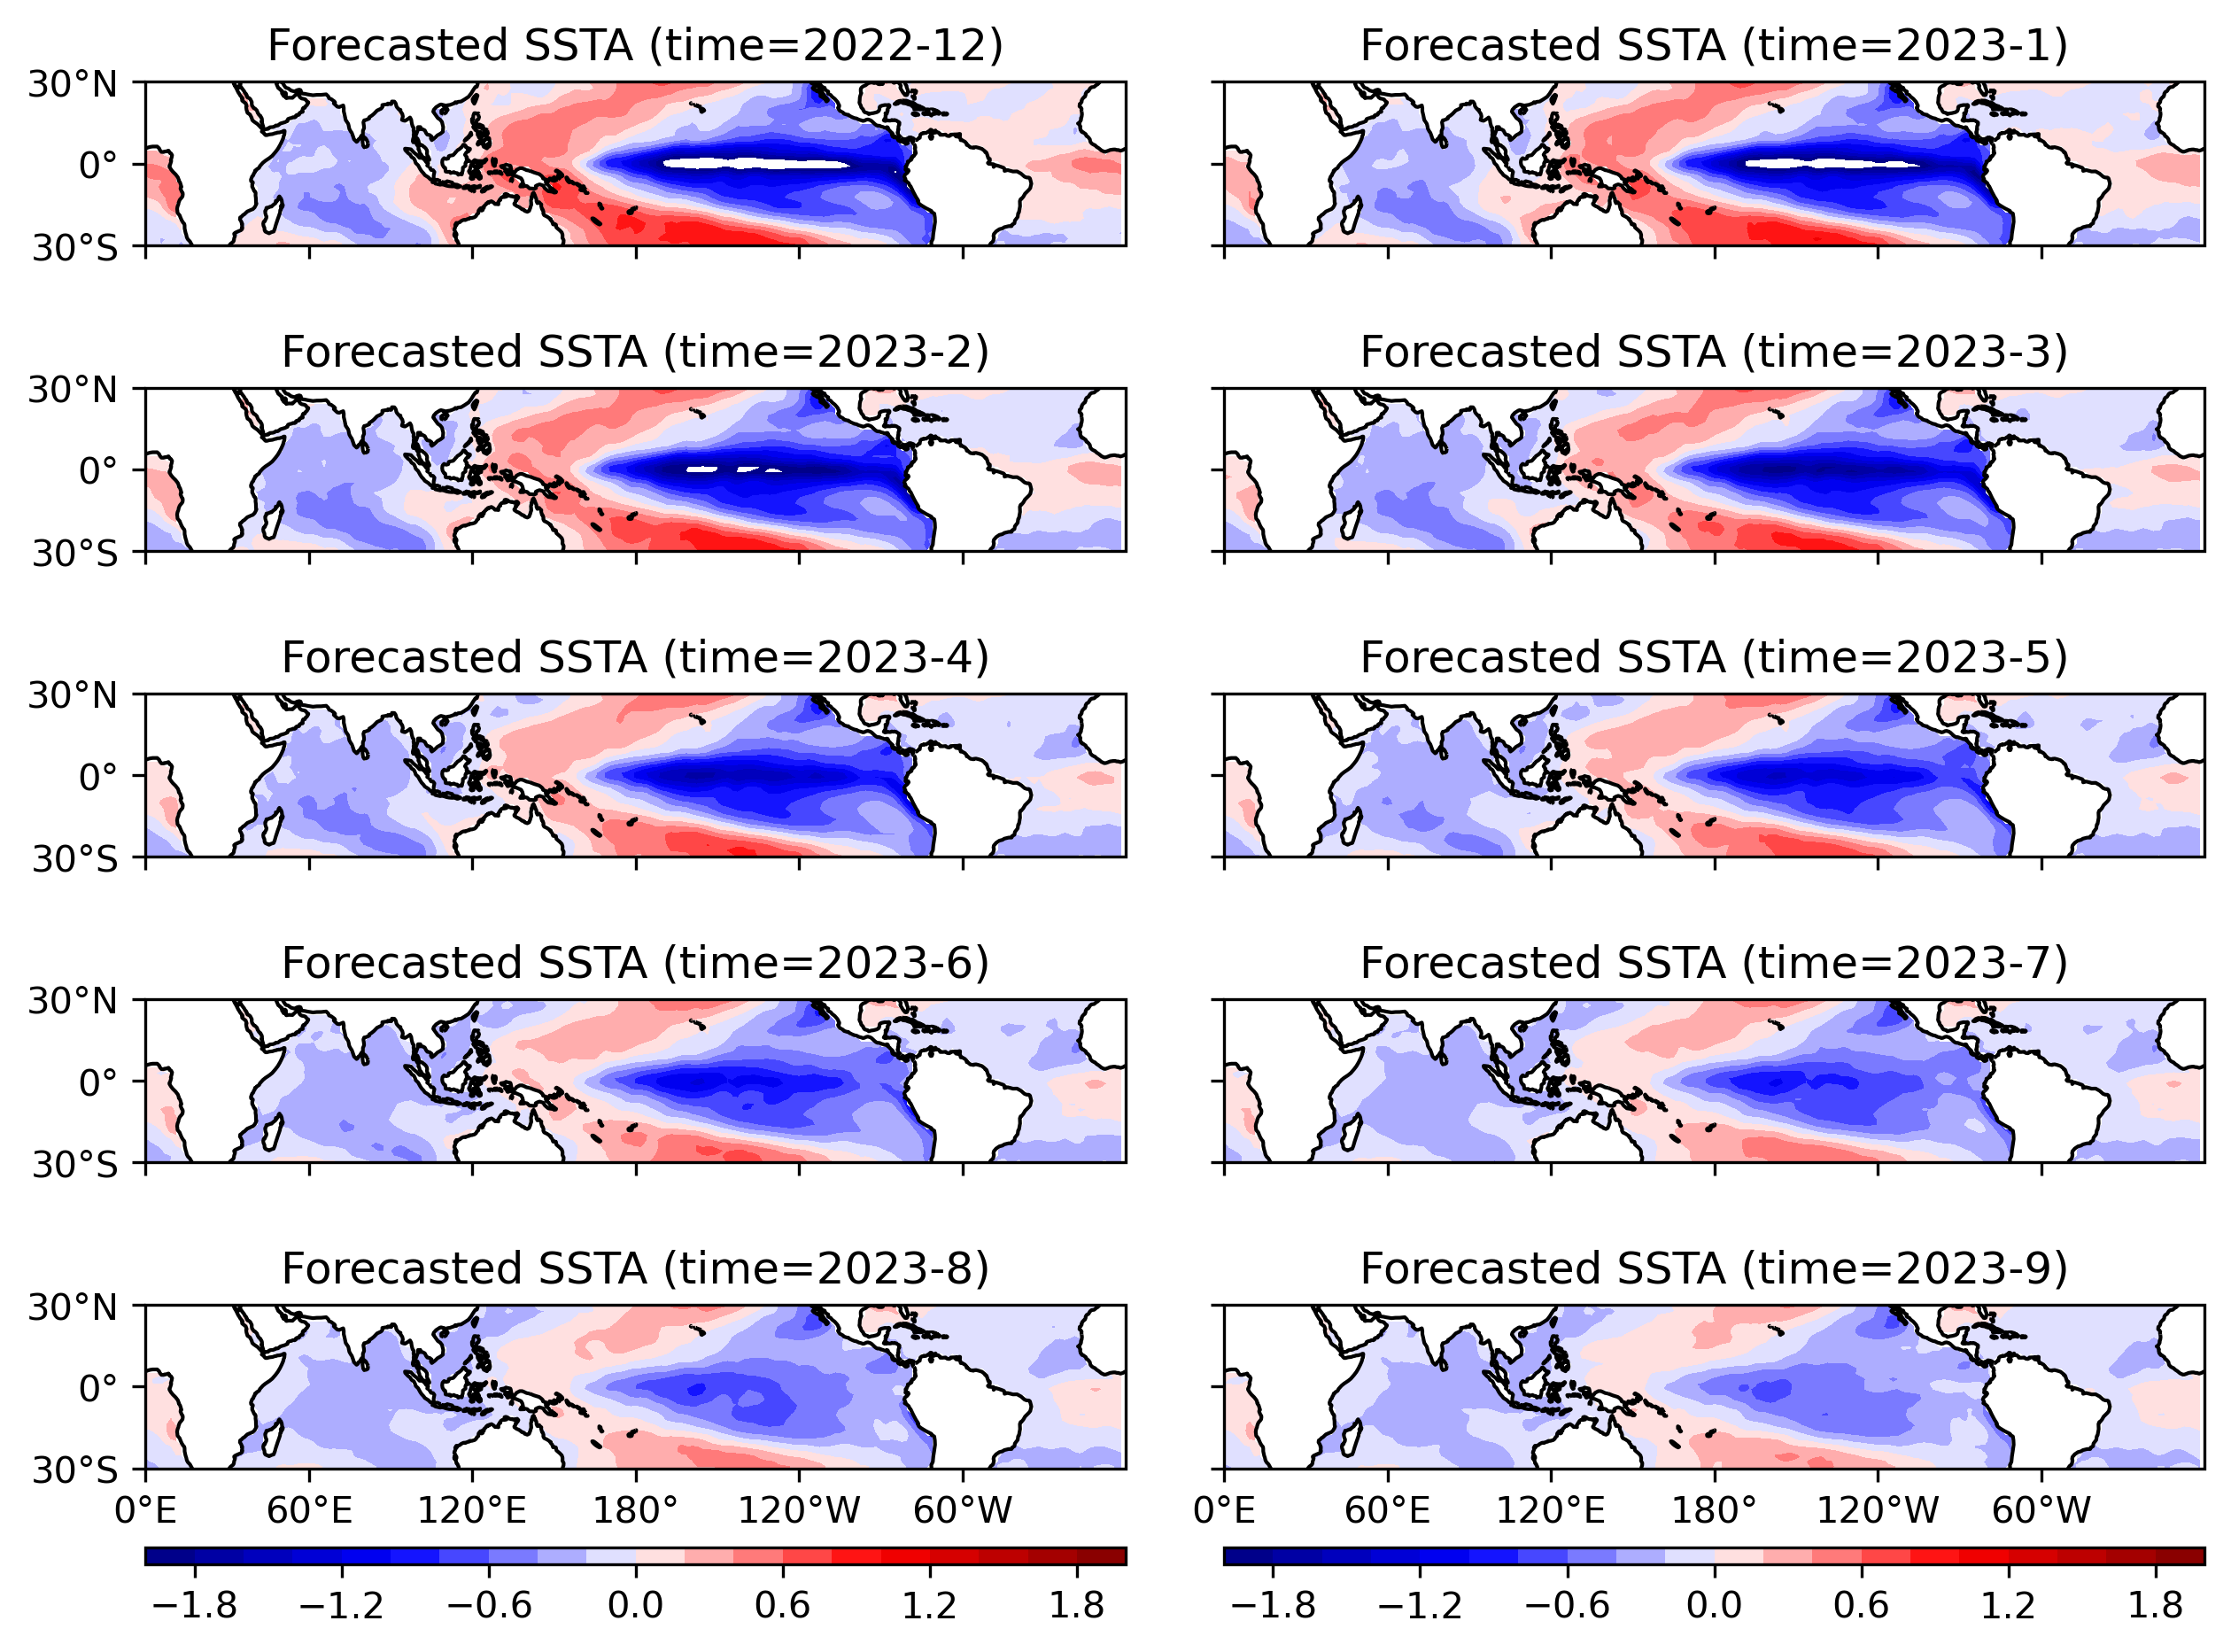
\includegraphics[width=\textwidth]{figures/forecasted_ssta_newest.png}
\caption{Forecasted SSTAs based on the latest SSTs.}
\label{fig:forecasted_ssta_newest}
\end{figure}

Fig. \ref{fig:forecasted_ssta_newest} shows the forecasted SSTAs based on the latest SSTs. The inital SSTA are taken from the COBE SST dataset. To get the anomalies, we use the latest 20 years data to calculate the climatology. From the forecasted SSTA map, we can see we are in a La Ni\~na event. And the in next 10 months, the La Ni\~na event is likely to continue. But due to the LIM is not accurate when forecasting the far future SSTAs, we do not have much confidence on the SSTAs in the later spring in next year. Futhermore, because of the existence of the "ENSO spring barrier", it is hard to predict the SSTAs in the later spring in next year.

\section{Conclusion and discussion}\label{conclusion}

In this project, we build a linear inverse model (LIM) to predict the SSTAs in the global tropics. The LIM is built in the EOF space. The LIM is accurate when forecasting the near future SSTAs, but not accurate when forecasting the far future SSTAs. The LIM is accurate in the Ni\~no 3 region and the Indian Ocean, but not accurate in the north Atlantic (especially in the Mexico Gulf) and tropical Atlantic. In the Northwest Pacific, the LIM also perform poorly. This is because the LIM is built based on EOF decomposition, and the strongest EOF mode is the ENSO. Therefore, the LIM can capture the ENSO signal well, but cannot capture the other signals well.

\section{Aknowledgements}\label{acknowledgements}

Thanks to Dr. Ping Chang for providing the datasets and the guidance. Thanks to Ms. Qiuying Zhang for helping me with the debugging of the Python script.

\bibliographystyle{abbrv}
\bibliography{library}

\end{document}
